\documentclass[red]{beamer}
\usetheme{Berkeley}
\usepackage{adjustbox}
\usepackage{graphicx}
\setbeamertemplate{footline}[frame number]{}
\defbeamertemplate*{footline}{noslidenum theme}



\title{“The Effect of Ambiguity on Price Dispersion in Duopoly Markets”}
\author{Zachary Dorobiala }
\institute{University of Alabama}
\date{EC698 November, 2021}

%/ *****TITLE SLIDE*****
\begin{document}
\begin{frame}
\titlepage
\end{frame}





%/ *****RESEARCH QUESTION SLIDE*****
\section{Research Q}
\begin{frame} [t]
\frametitle{Research Question}
\underline{Research Question:} \\~\\
\hspace*{20pt} How does ambiguity about market share effect price dispersion in duopoly markets? \\~\\ \\~\\
\underline{Experimental Prediction} \\~\\
\hspace*{20pt} If sellers are averse to ambiguity we would expect sellers to decrease dispersion with the introduction of ambiguity.
\end{frame}




%/ *****MODEL/LITERATURE SLIDE(1)*****
\section{Model/Lit}
\begin{frame} [t]
\frametitle{Baseline Model / Literature}
\underline{Doupoly Pricing Model:} \\~\\
- Informed ($\psi_0$) and Captive ($\psi_1$, $\psi_2$) \\
- Unit demand of one homogeneous product with MC=0\\
- Reservation price set to 1 \\
- Constraint: $\psi_0 + \psi_1 + \psi_2 = 1$ \\
- If $\psi_1 > \psi_2$, then Firm 1 uses the mixed strategy H(p) and Firm 2 uses the mixed strategy G(p) \\~\\

\underline{Literature:} \\~\\
\textbf{Symmetric}: Salop and Stiglitz (1977), Shilony (1977), Rosenthal (1980), Varian (1980)\\
\textbf{Asymmetric}: Baye and Morgan (2001), Morgan et al. (2006), Chioveanu (2008)\\
\end{frame}





%/ *****MOTIVATION SLIDE*****
\section{Background/ Motivation}
\begin{frame} [t]
\frametitle{Background/ Motivation}
Risk v. Ambiguity \\~\\ \\~\\

How pricing markets in practice deviate from the literature. \\~\\ \\~\\



 Tversky and Fox (1995) stated that ambiguity has recently attracted much attention because many agents and firms make decisions without precise knowledge of how probabilistic those decisions outcomes will be. They note that decisions like going into business, going to court, or going into medical surgery are all decided in the absence of precise probabilities. \\~\\ \\~\\
 
 Increased price competition. 
\end{frame}







%/ *****MODEL/LITERATURE SLIDE(2)*****
\begin{frame} [t]
\frametitle{Model/ Preferences}
\underline{Ambiguity Preferences}\\~\\
The $\alpha$-maximin preferences can be written as:
\begin{multline}
    V_i (p; \psi_i, \alpha_i, A_i) = \alpha_i [\underset{\psi_{i} \in A_{i}}{Max}\; E\pi_i(H(p), G(p), \psi_i)] \\ \hspace*{100pt} + (1 - \alpha_i) [\underset{\psi_{i} \in A_{i}}{Min}\; E\pi_i(H(p), G(p), \psi_i)] 
    \label{VV}
\end{multline}
\\
\underline{Comparative Statics}
\begin{equation}
    \frac{\partial E(p_1)}{\partial \alpha_1} > 0 \hspace*{45pt} \frac{\partial E(p_2)}{\partial \alpha_2} < 0
\end{equation}
\end{frame}






%/ *****EXPERIMENTAL DESIGN SLIDE(1)*****
\begin{frame} [t]
\section{Design}
\frametitle{Experimental Design}
\begin{itemize}
\setlength{\itemsep}{20pt}
    \item Experiment uses a 2x2 between-subjects design \\
    \hspace*{30pt} 1) Change in informed consumer shares ($\psi_0$) \\
    \hspace*{30pt} 2) Ambiguity on the captive consumer shares\\
    \item $\psi_0$ varied at 20\% (Low) and 60\% (High) of the total consumer continuum. If ambiguity was not present within the captive consumer shares (No), if so (Yes). Ambiguity was presented to subjects as a range (A\%, B\%). Two-letter combination: LN, LY, HN, HY. \\
    
    \item The experiment consists of 24 sessions at the University of Alabama, TIDE Lab, in the Spring of 2021. All choices and information are entered into the z-Tree program, Fischbacher, U (2007).
\end{itemize}
\end{frame}





%/ *****EXPERIMENTAL DESIGN SLIDE(1.5)*****
\begin{frame} [t]
\frametitle{Procedures}
\begin{itemize}
    \item 24 Sessions / 6 Subjects / 25 Pricing markets (35 period realizations) 
    \\~\\
    \item Random re-matching after each market
    \\~\\
    \item Each subject entered a distribution instead of a single price
    \\~\\
    \item 60-minute session
    \\~\\
    \item Average earnings in study was \$20.39
\end{itemize}
\end{frame}






%/ *****EXPERIMENTAL DESIGN SLIDE(1.8)*****
\begin{frame} [t]
\frametitle{Decision z-Tree Page}
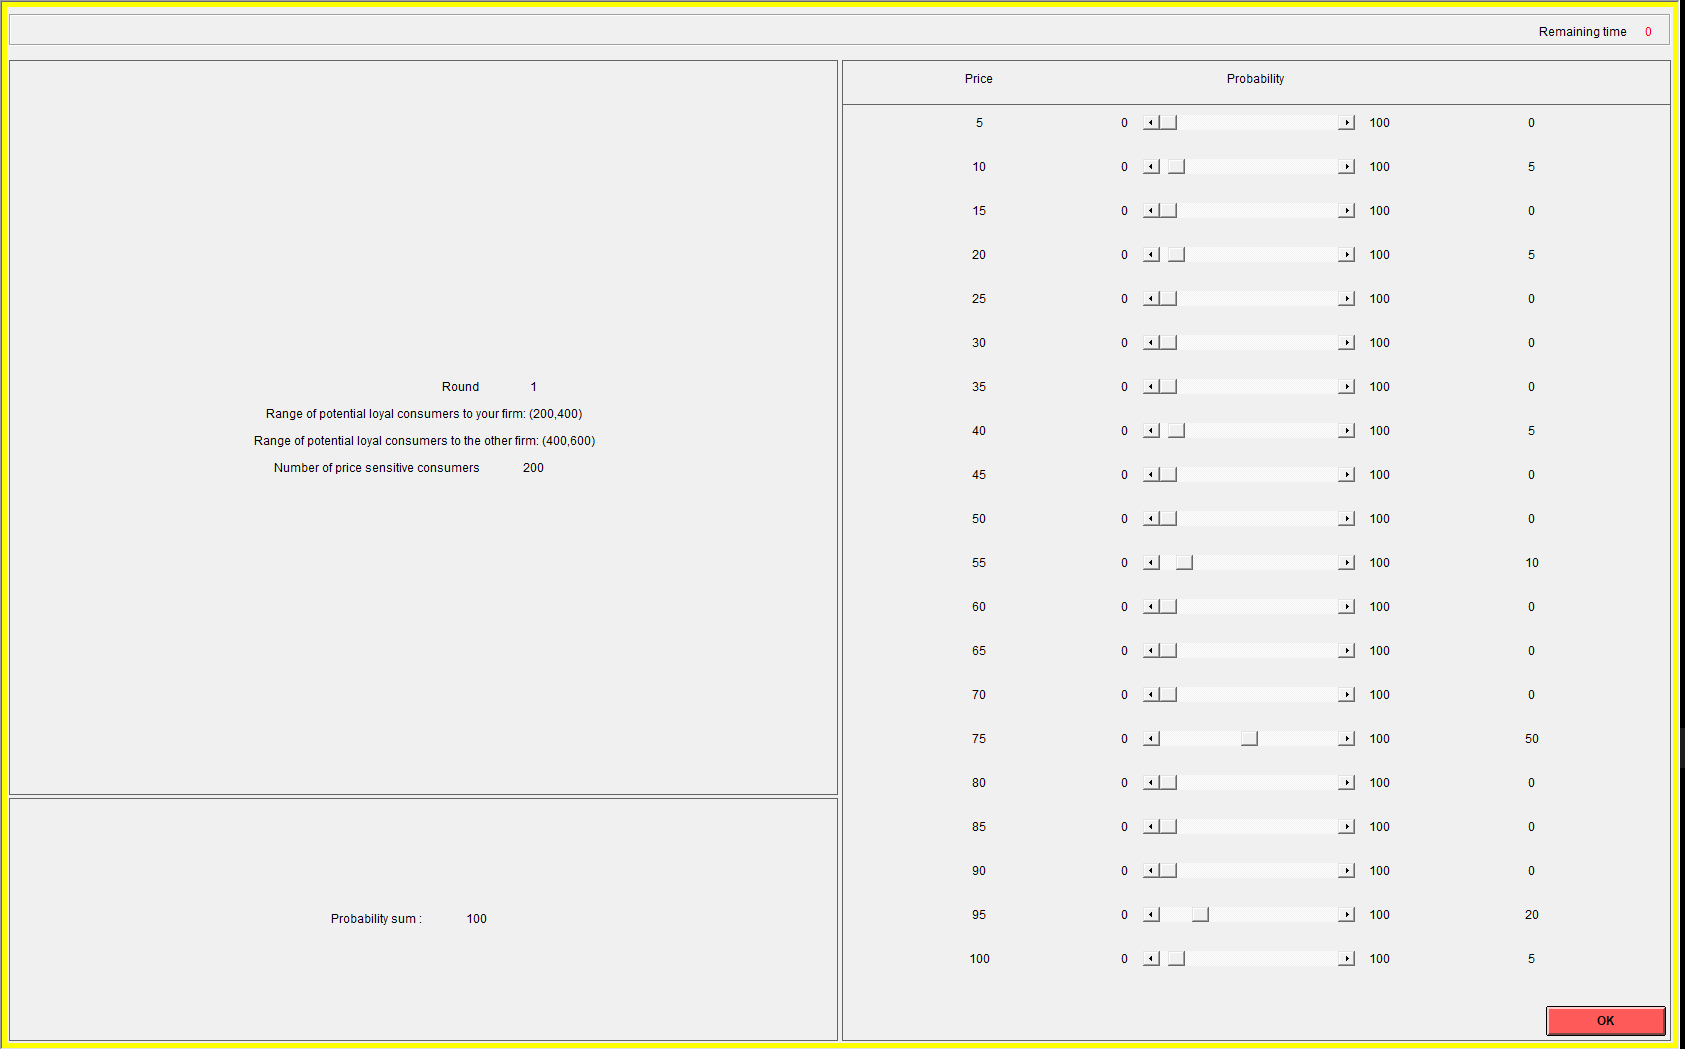
\includegraphics[width=10cm,height=7cm]{Decision.png}
\end{frame}





%/ *****EXPERIMENTAL DESIGN SLIDE(1.9)*****
\begin{frame} [t]
\frametitle{Result z-Tree Page}
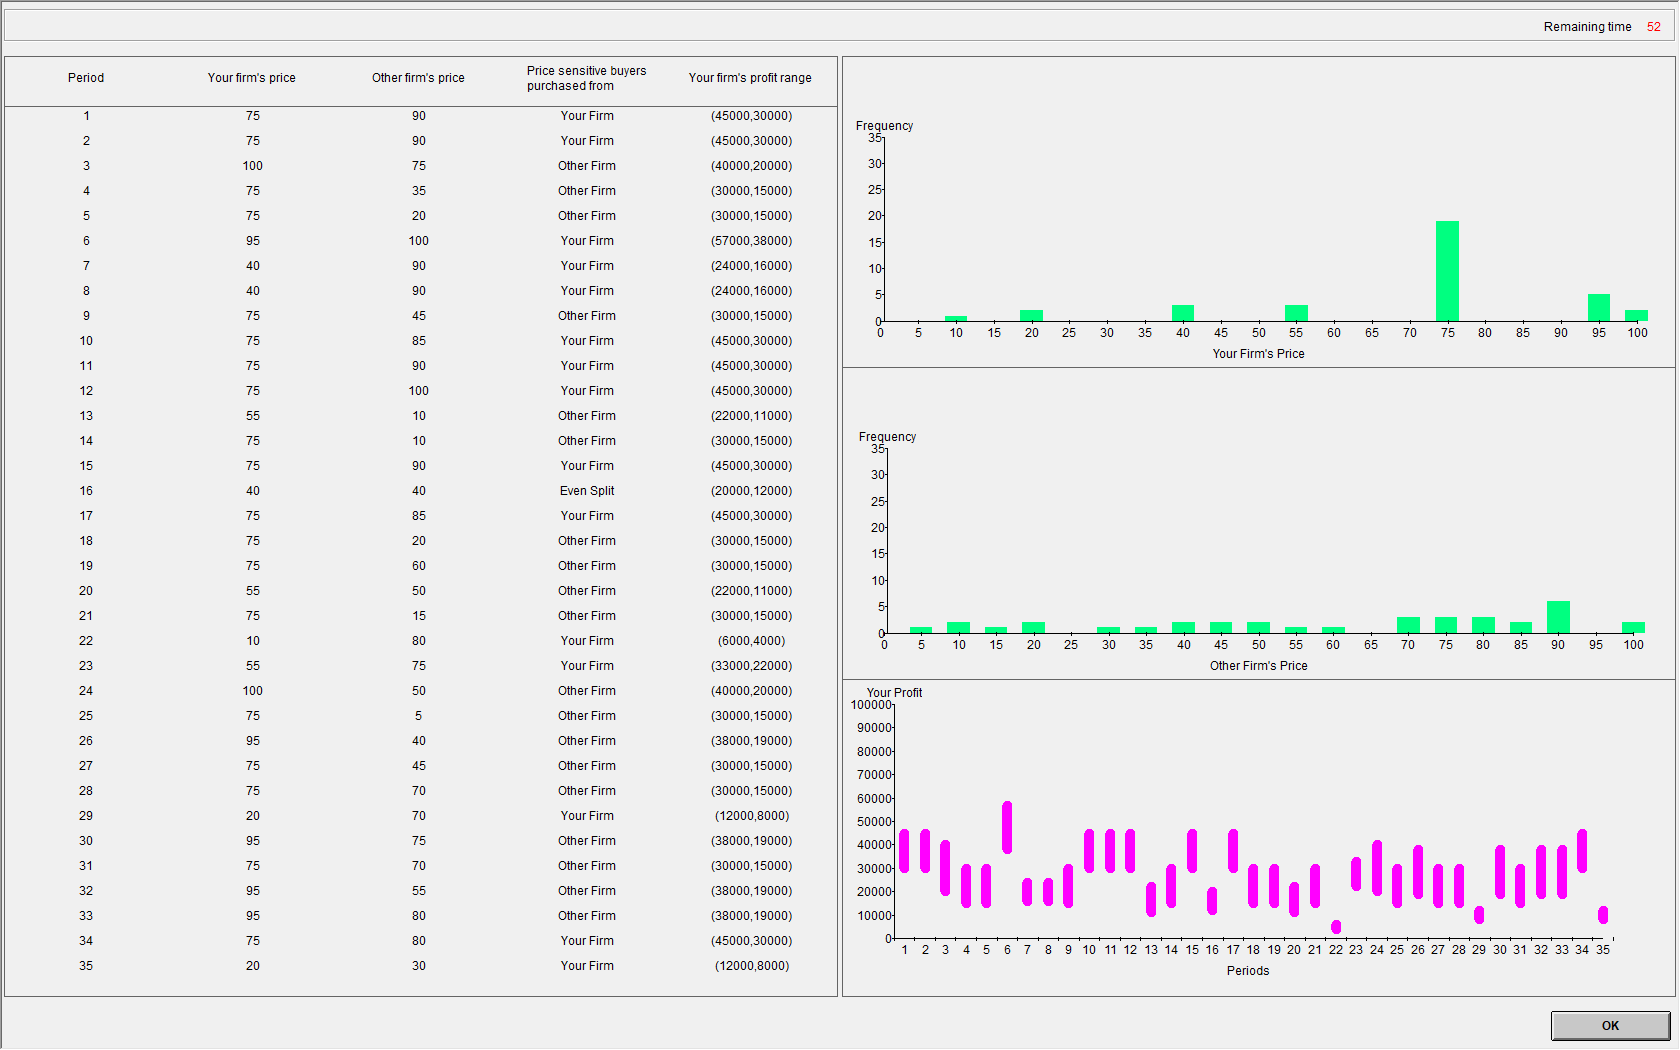
\includegraphics[width=10cm,height=7cm]{Result.png}
\end{frame}




%/ *****EXPERIMENTAL DESIGN SLIDE(2)*****
\begin{frame} [t]
\frametitle{Design Predictions: Unambiguous Captive Consumers}
\begin{figure} [h] 
\begin{center}
\begin{tabular}{c c}
\underline{LN Treatment} & \underline{HN Treatment} \\
$\psi_0 = 20\%$ & $\psi_0 = 60\%$ \\
$\psi_1 = 50\%$ & $\psi_1 = 30\%$ \\
$\psi_2 = 30\%$ & $\psi_2 = 10\%$ \\
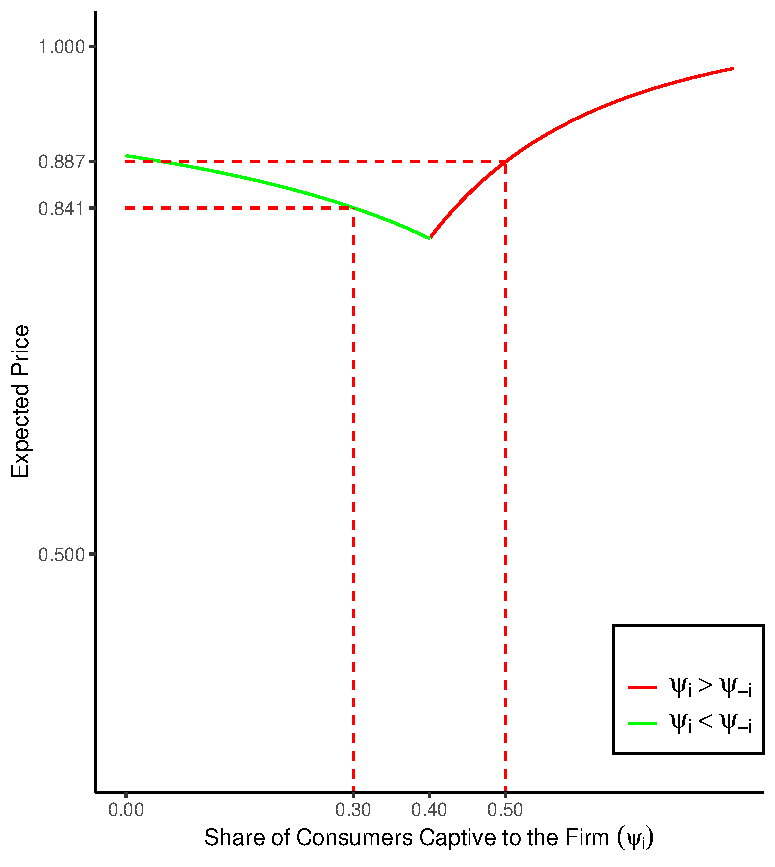
\includegraphics[width=5cm,height=5cm]{AA20 (1).pdf} & 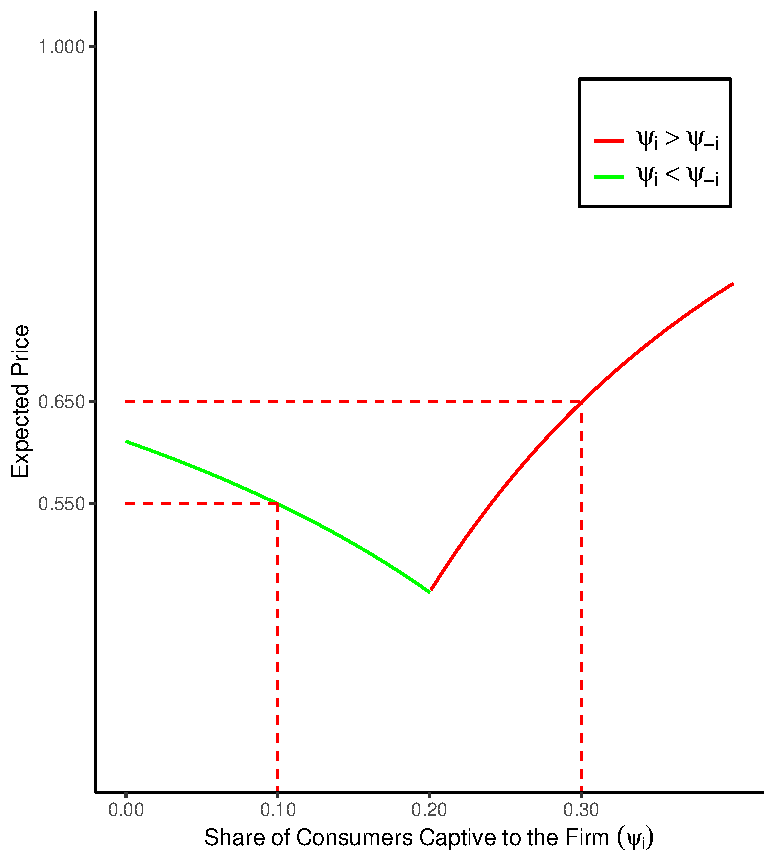
\includegraphics[width=5cm,height=5cm]{AA60 (1).pdf}
\end{tabular}
\end{center}
\end{figure}
\end{frame}





%/ *****EXPERIMENTAL DESIGN SLIDE(3)*****
\begin{frame} [t]
\frametitle{Design Predictions:Ambiguous Captive Consumers}
\begin{figure} [h] 
\begin{center}
\begin{tabular}{c c}
\underline{LY Treatment} & \underline{HY Treatment} \\
$\psi_0 = 20\%$ & $\psi_0 = 60\%$ \\
$\psi_1 \in [40\%, 60\%]$ & $\psi_1 \in [20\%, 40\%]$ \\
$\psi_2 \in [20\%, 40\%]$ & $\psi_2 \in [0\%, 20\%]$ \\
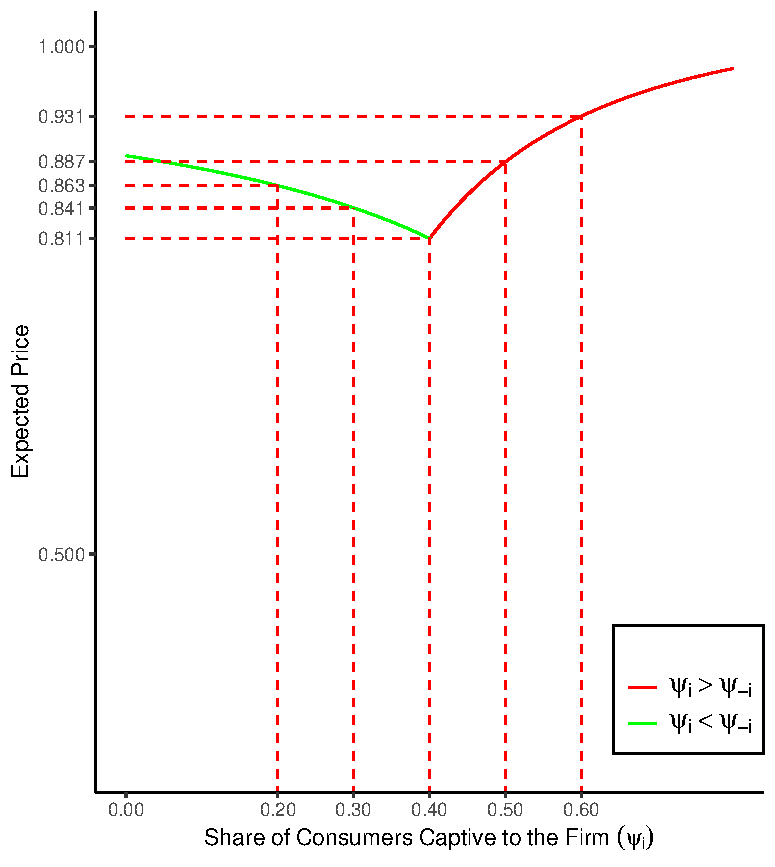
\includegraphics[width=5cm,height=5cm]{A20 (1).pdf} & 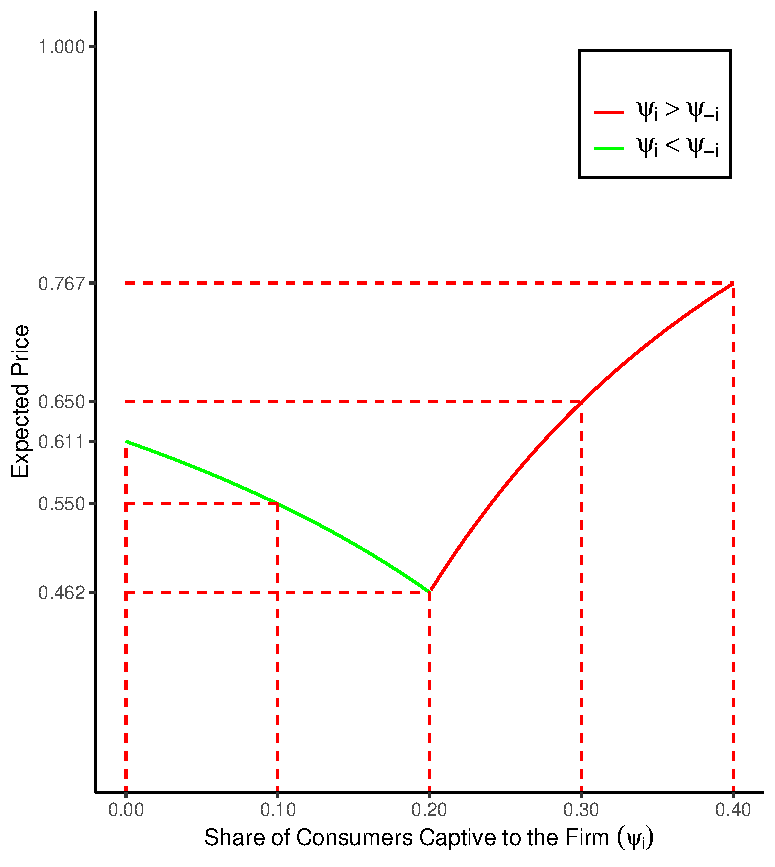
\includegraphics[width=5cm,height=5cm]{A60 (1).pdf}
\end{tabular}
\end{center}
\end{figure}
\end{frame}





%/ *****RESULTS SLIDE(1)*****
\begin{frame}
\section{Results}
\frametitle{Treatment Market Price by Period}
\begin{center}
    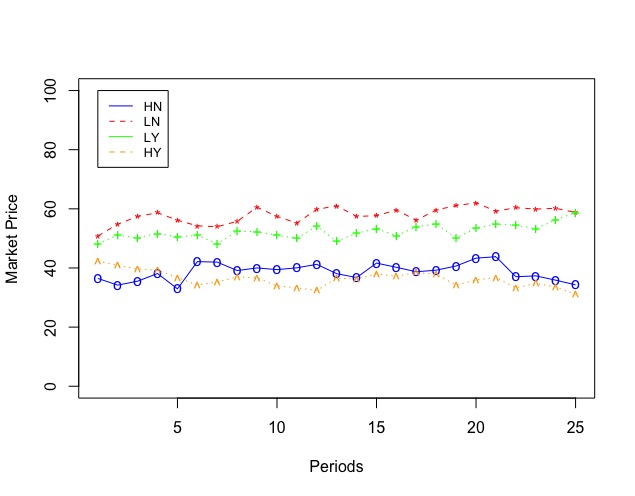
\includegraphics[width=10cm,height=8cm]{Mktprice by TREATMENT (1).jpeg}
\end{center}
\end{frame}






%/ *****RESULTS SLIDE(2)*****
\begin{frame}
\frametitle{Increasing Informed Consumer Share}
\newcommand{\adv}[1]{ {\color{blue} #1} }
\begin{table}[htbp]\centering
 \begin{adjustbox}{width=10cm, totalheight=7cm}
\begin{tabular}{l*{2}{c}}
\hline\hline
Market Price  & (1) & \\
\hline
Period                                      &  0.09 & \\
                                            &  (0.10) & \\
HighInformed                                &  \adv{ -19.19$^{***}$} &\\
                                            &  (5.76)& \\
Ambiguity                                &  \textcolor{red}{-5.69} &\\
                                            &  (7.10) & \\
HighInformed $\times$ Ambiguity   & 3.18 & \\
                                            &  (9.07) &\\
Constant                                    & 56.76$^{***}$ & \\
                                            &  (4.85) & \\
\hline 
\vspace{2mm}
$R^2$                                       & 0.19 &  \\
Observations                                &   3600 &  \\
\hline\hline
Null Hypothesis                             & Two-sided p-value \\
\hline
Ambiguity + HighInformed  $\times$ Ambiguity = 0 & \textcolor{red}{0.66} \\
\hline
\multicolumn{2}{l}{\footnotesize{Note: Standard errors are in parenthesis and are clustered at the session level.}} \\
\multicolumn{2}{l}{\footnotesize{Significance levels: * p $<$ 0.10, ** p $<$ 0.05, *** p $<$ 0.01.}}
\end{tabular} \\ \vspace{3mm}
 \end{adjustbox}
\end{table}
\end{frame}





%/ *****RESULTS SLIDE(3)*****
\begin{frame}
\frametitle{Dispersion by Treatment}
\begin{table}[htbp]\centering
 \begin{adjustbox}{width=10cm, totalheight=7cm}
\begin{tabular}{l*{2}{c}}
\hline\hline
Dispersion  & (1) & \\
\hline
Period                                      &  0.29$^{***}$  & \\
                                            &  (0.11) & \\
HighInformed            &   0.35 &\\
                                            &  (4.66)& \\
Ambiguity                                   &  \textcolor{red}{.79} &\\
                                            &  (3.81) & \\
HighInformed  $\times$ Ambiguity    & -11.34$^{*}$ & \\
                                            &  (6.59) &\\
Constant                                    & 25.34$^{***}$ & \\
                                            &  (2.86) & \\
\hline 
\vspace{2mm}
$R^2$                                       & 0.05 &  \\
Observations                                &   3600 &  \\
\hline\hline
Null Hypothesis                             & Two-sided p-value \\
\hline
Ambiguity + HighInformed  $\times$ Ambiguity = 0 & \textcolor{red}{0.05} \\
\hline
\multicolumn{2}{l}{\footnotesize{Note: Standard errors are in parenthesis and are clustered at the session level.}} \\
\multicolumn{2}{l}{\footnotesize{Significance levels: * p $<$ 0.10, ** p $<$ 0.05, *** p $<$ 0.01.}}
\end{tabular} \\ \vspace{3mm}
 \end{adjustbox}
\end{table}
\end{frame}





%/ *****RESULTS SLIDE(4)*****
\begin{frame}
\frametitle{HN / HY}
\begin{figure} [h] 
\begin{center}
\begin{tabular}{c c}
HN & HY \\
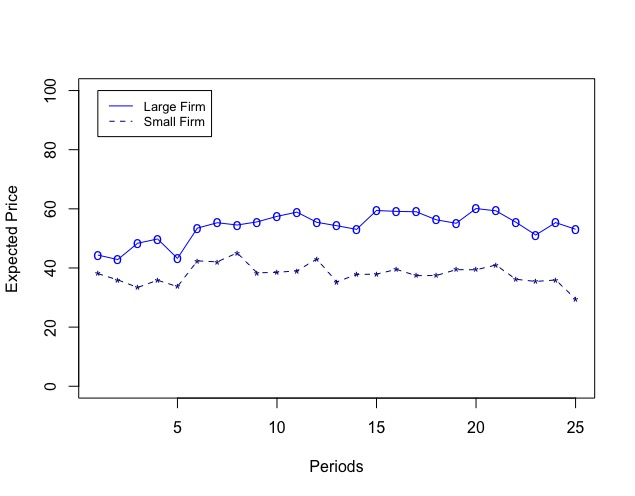
\includegraphics[width=5cm,height=4cm]{HN - FIRM (1).jpeg} & 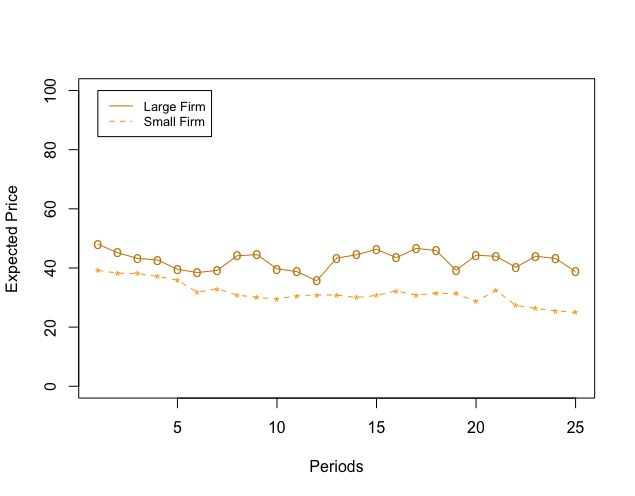
\includegraphics[width=5cm,height=4cm]{HY - FIRM (1).jpeg}
\end{tabular}
\end{center}
\end{figure}
\begin{center}
 \begin{adjustbox}{width=10cm, totalheight=1.5cm}
\begin{tabular}{ |c|c|c|c|c| } 
 \hline
   & HN: Small & HY: Small & HN: Large & HY: Large &
    \cline{1-5}
   Avg. Price & \textcolor{blue}{36 } & \textcolor{orange}{31.5} &  \textcolor{blue}{ 54} & \textcolor{orange}{41} \\
   \cline{1-5}
 \hline
\end{tabular}
 \end{adjustbox}
\end{center}
\end{frame}





%/ *****RESULTS SLIDE(5)*****
\begin{frame}
\frametitle{HN / HY}
\begin{figure} [h] 
\begin{center}
\begin{tabular}{c c}
HN: Small & HN: Large \\
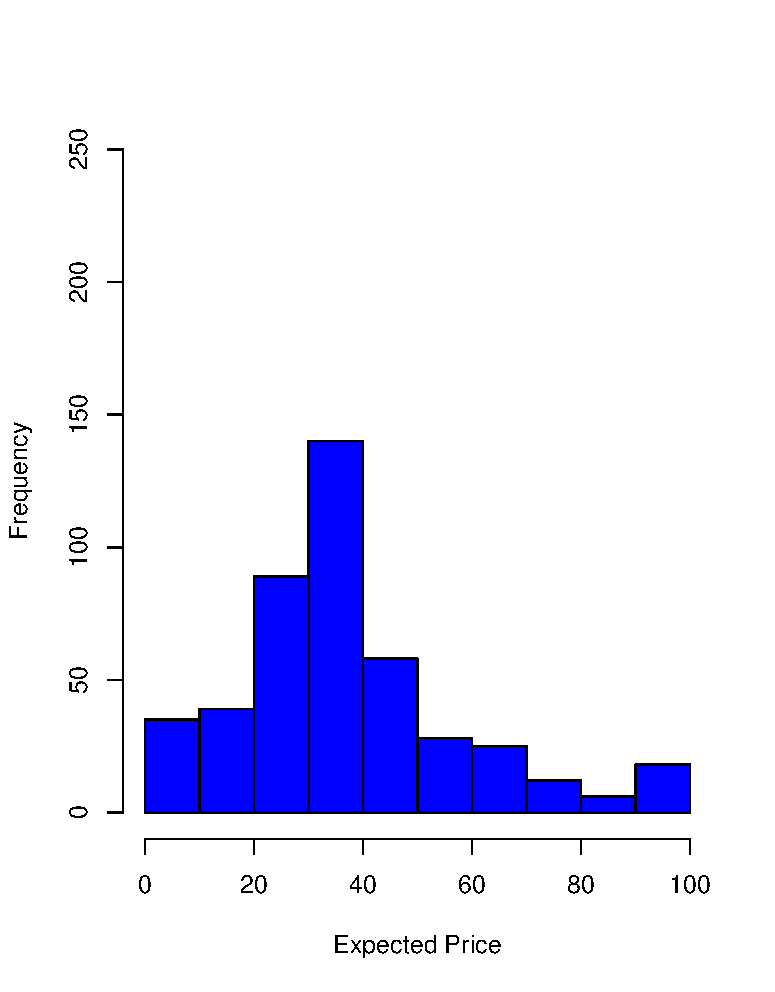
\includegraphics[width = 5cm, height = 3.1cm]{HSN (1) (1).pdf} &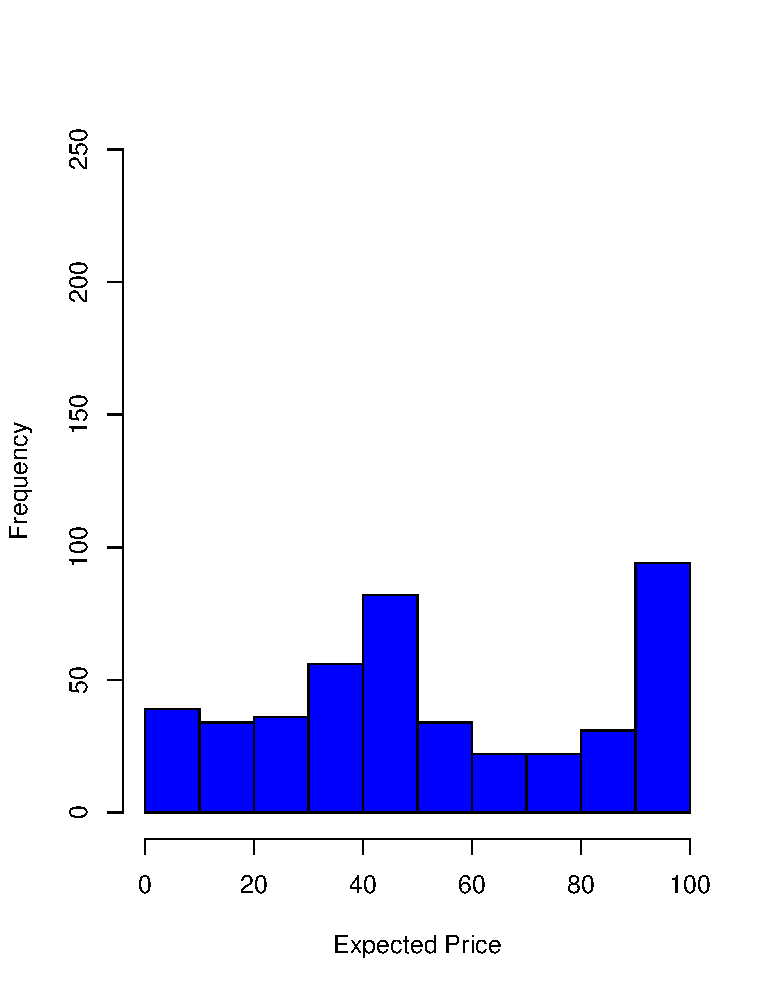
\includegraphics[width = 5cm, height = 3.1cm]{HLN (1) (1).pdf} \\
HY: Small & HY: Large \\
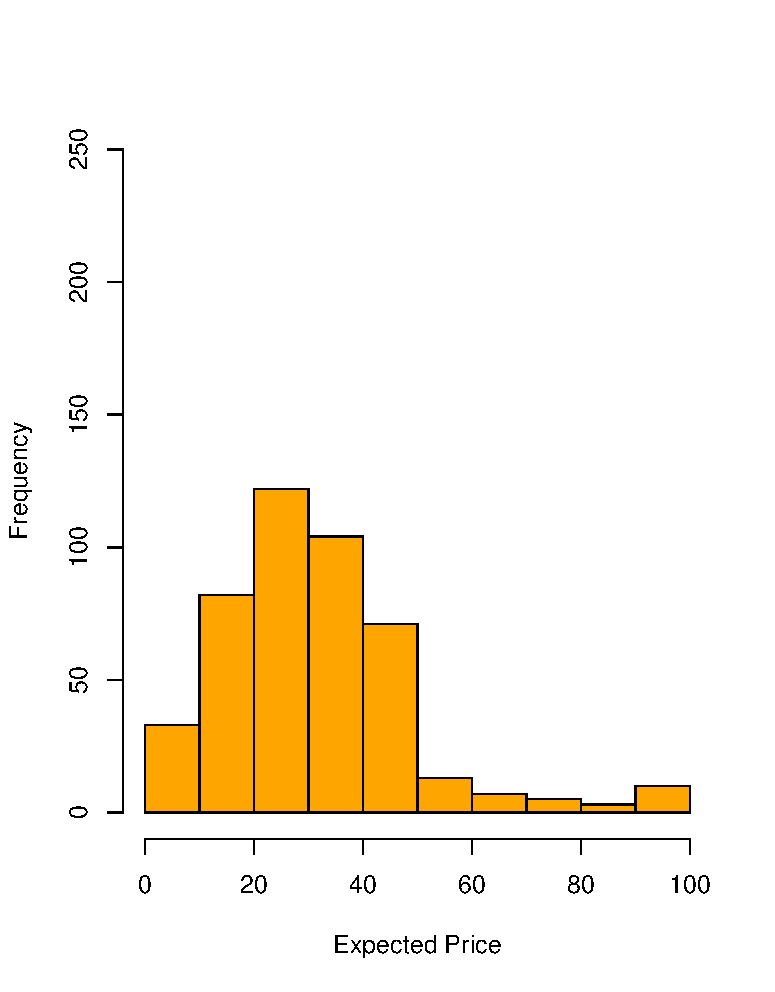
\includegraphics[width = 5cm, height = 3.1cm]{HSY (1) (1).pdf} & 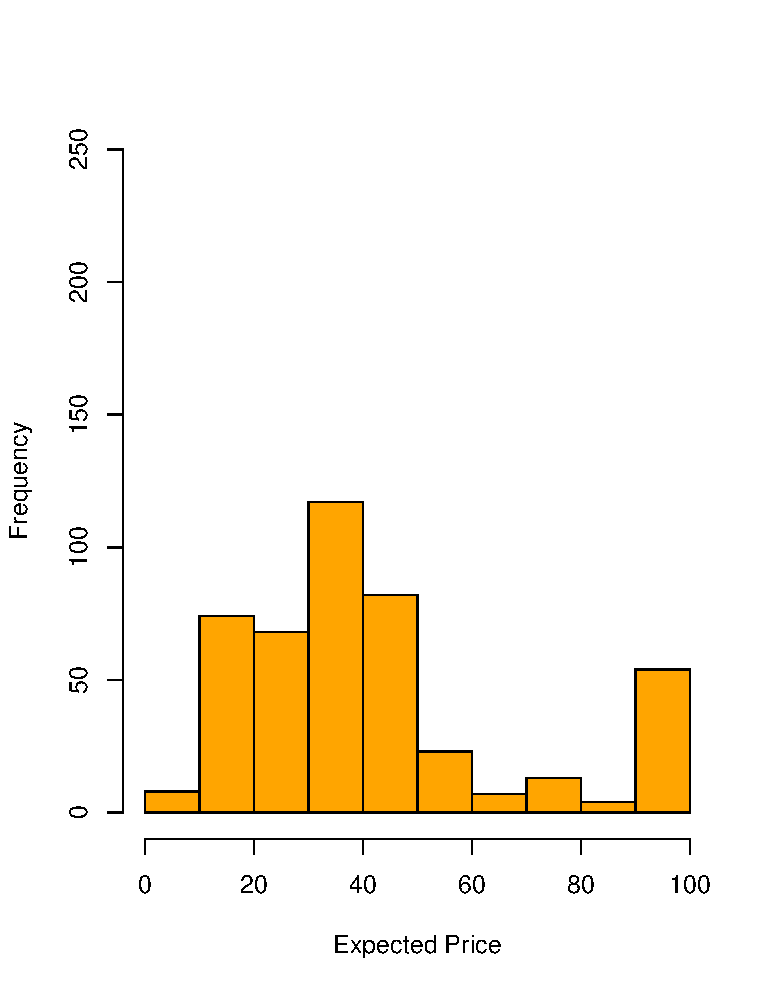
\includegraphics[width = 5cm, height = 3.1cm]{HLY (1) (1).pdf}
\end{tabular}
\end{center}
\end{figure}
\end{frame}





%/ *****FINDINGS SLIDE*****
\section{Summary}
\begin{frame} [t]
\frametitle{Summary}
\underline{Findings:} \\~\\
\hspace*{20pt} 1) The effect of ambiguity on average price \\~\\ \\~\\  

\hspace*{20pt} 2) The effect of ambiguity on Low and High markets \\~\\ \\~\\ 

\hspace*{20pt} 3) The effect of ambiguity on Large and Small firms \\~\\ \\~\\ 
\end{frame}





%/ *****Thank You SLIDE*****
\begin{frame} [t]
\frametitle{}
\vspace*{80pt}
\centering{Thank You and Roll Tide!}
\end{frame}




%%/ *****EXTRA SLIDE*****
%\begin{frame}
%\frametitle{LN / LY}
%\begin{figure} [h] 
%\begin{center}
%\begin{tabular}{c c}
%LN & LY \\
%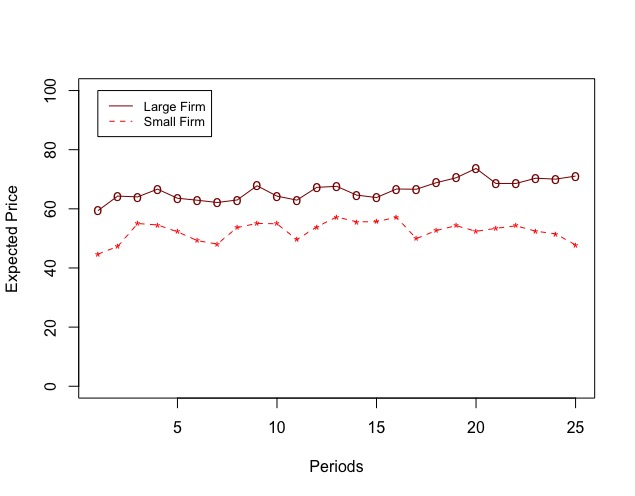
\includegraphics[width=5cm,height=4.5cm]{LN - FIRM (1).jpeg}
%& 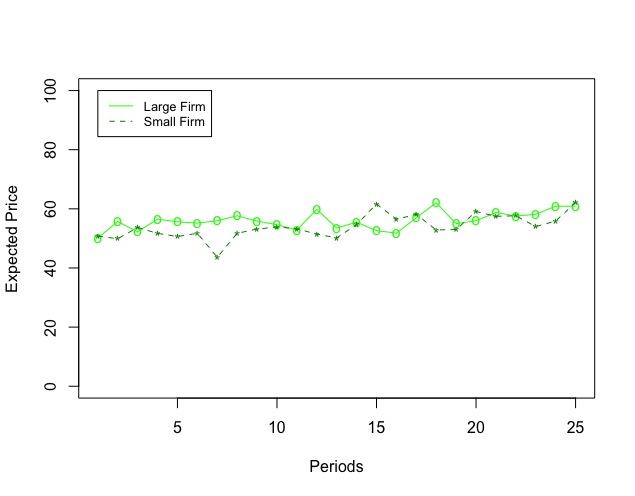
\includegraphics[width=5cm,height=4.5cm]{LY - FIRM (1).jpeg}
%\end{tabular}
%\end{center}
%\end{figure}
%\begin{center}
% \begin{adjustbox}{width=10cm, totalheight=1.5cm}
%\begin{tabular}{ |c|c|c|c|c| } 
% \hline
%  & LN: Small & LY: Small & LN: Large & LY: Large &
%    \cline{1-5}
%   Avg. Prices &\textcolor{red}{48.7}& \textcolor{green}{50.4} &\textcolor{red}{65.5} & \textcolor{green}{55.9} \\
% \hline
%\end{tabular}
% \end{adjustbox}
%\end{center}
%\end{frame}
%
%\begin{frame}
%\frametitle{LN / LY}
%\begin{figure} [h] 
%\begin{center}
%\begin{tabular}{c c}
%LN: Small & LN: Large \\
%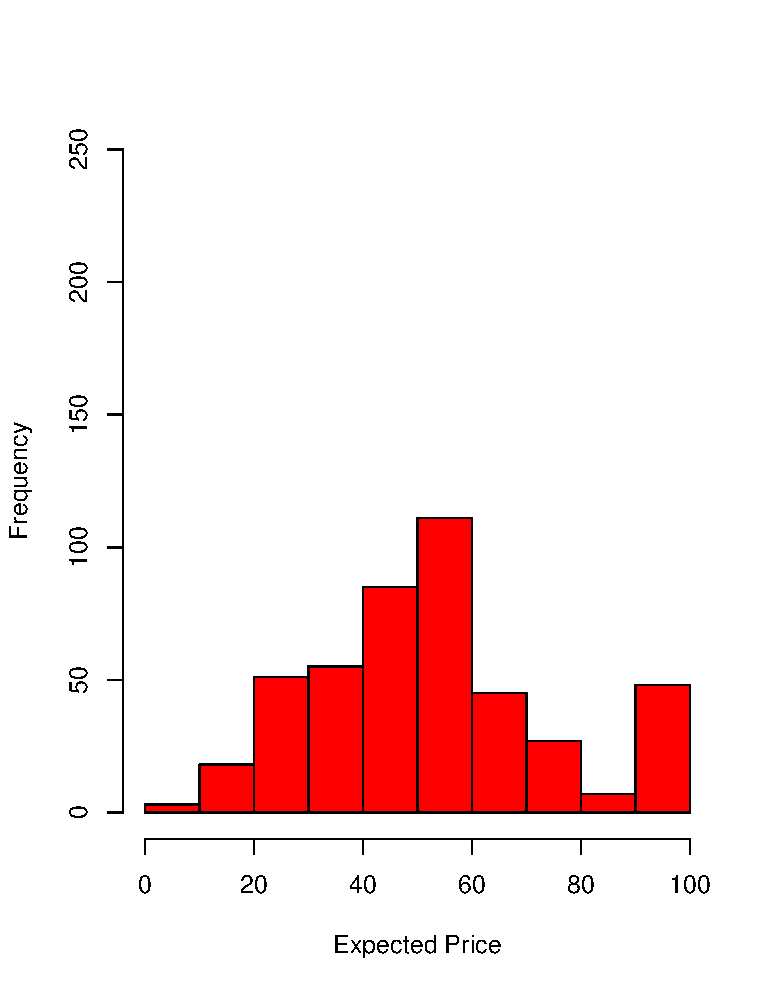
\includegraphics[width = 5cm, height = 3.1cm]{LSN (1) (1).pdf}
%& 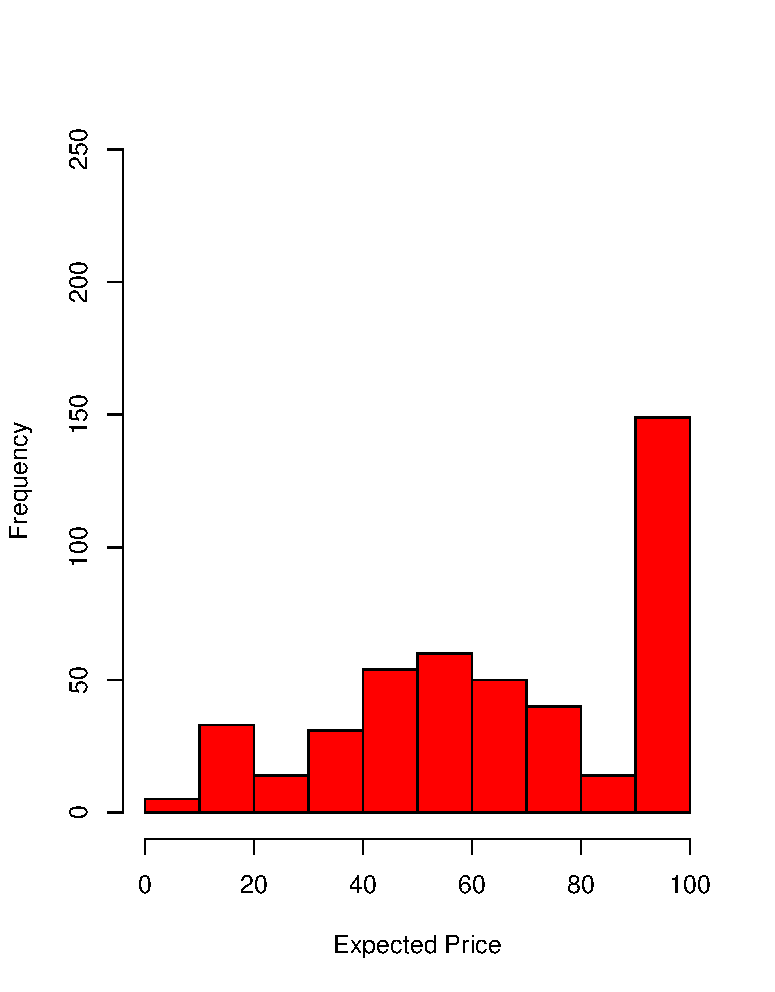
\includegraphics[width = 5cm, height = 3.1cm]{LLN (1) (1).pdf}\\
%LY: Small & LY: Large \\
%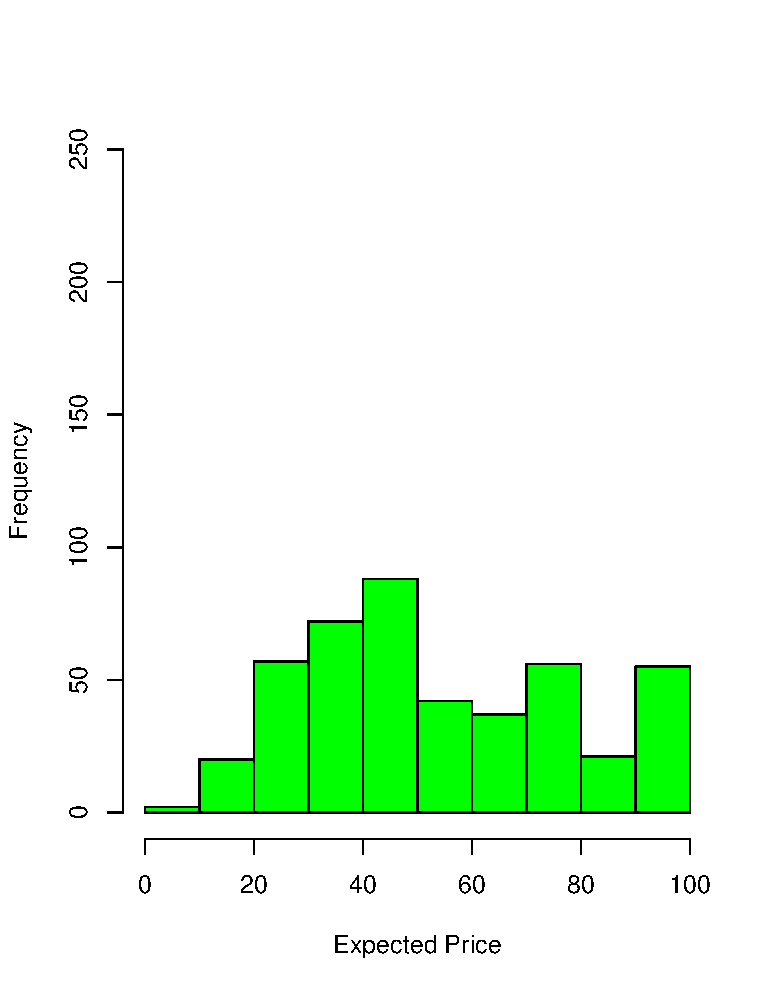
\includegraphics[width = 5cm, height = 3.1cm]{LSY (1) (1).pdf}
%& 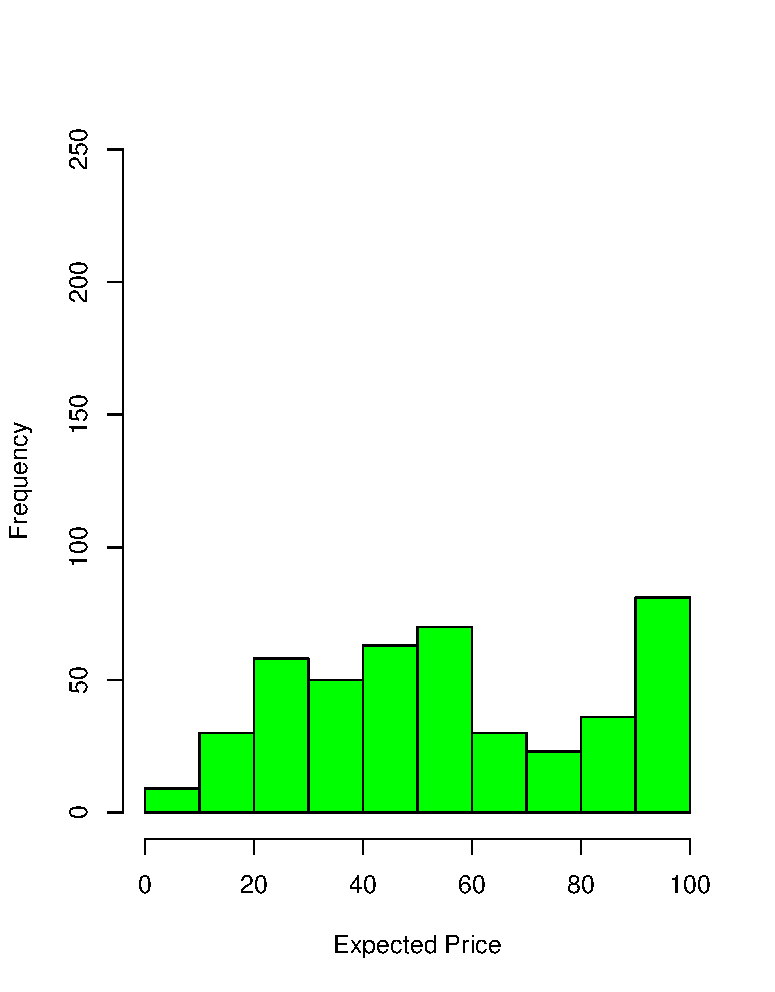
\includegraphics[width = 5cm, height = 3.1cm]{LLY (1) (1).pdf}
%\end{tabular}
%\end{center}
%\end{figure}
%\end{frame}

\end{document}
